\chapter{Evaluation} \label{chp:Evaluation}
In this chapter we want to present and discuss our evaluation results. Using Baselines Lab, we perform tests in a variety of different scenarios. After explaining our general test procedure in Section \ref{sec:TestProcedure}, we will begin, by evaluating the basic components for solving maze environments. In Section \ref{sec:EvalReward} we will take a look at reward generation and continue with a deeper look into observation generation and preprocessing in Section \ref{sec:EvalObs}. Section \ref{sec:EvalRLAlgorithms} will shine some light on the question which learning algorithm performs best when dealing with our particle navigation task and we will wrap up the evaluation of the basic parameters in Section \ref{sec:EvalParameters} where we take a look at the influence of various RL hyperparameters.

The initial tests will allow us to generate a baseline for the performance of our model, which then will be used throughout the rest of the evaluation to compare the influence of other factors. We begin, by testing how much inaccuracy in both actions and observations will influence the agent in Section \ref{sec:EvalError} and continue with the extension of the particle model with physical particles in Section \ref{sec:EvalPhysical}. We will then take a look at randomized instances in Section \ref{sec:EvalRandomness} and finish with a comparison with algorithmic approaches in Section \ref{sec:EvalAlgorithms}.


\section{Test Procedure} \label{sec:TestProcedure}
In this section we want to talk about different aspects of our test procedure.

\paragraph{Environment.}
All experiments were done on a Linux workstation running Ubuntu 18.04 LTS. The workstation has an Intel 6700K CPU, a single Nvidia GeForce GTX 1080 Ti GPU and 64GB of main memory. We installed Python 3.7.3 using the Anaconda \cite{anaconda} software distribution. We also used Tensorflow 1.14 in conjunction with the CUDA Toolkit version 10.1.243 and CUDNN version 7.6.5. Baselines Lab was developed on top of Stable-Baselines 2.10 and NumPy 1.17. For a complete list of installed packages see Appendix TODO.

\paragraph{Procedure.}
Our experiments involved several sources of randomness. To ensure consistent executions, we fixed the random seed for all involved components to the same value for all experiments. Unfortunately Tensorflow 1.14 does not guarantee consistent results during GPU computations. We therefore repeated experiments three times and averaged the results for comparison. The learning curves provided in this chapter are also smoothed by a running average, using window containing the last 100 steps.

\paragraph{Initial Hyperparameters.}
For our initial experiments we wanted to use general purpose hyperparameters for the PPO algorithm. We therefore used parameters similar to the parameters used in the RND paper \cite{burda2018exploration} (see Table \ref{tab:RNDParameters}) which showed to produce good results across all Atari environments. 


\begin{table} [ht]
    \begin{center}
        \begin{tabular}{|c|c|}
            \hline
            Hyperparameter & Value \\
            \hline
            Rollout Length & 256 \\
            Number of minibatches & 8 \\
            Number of optimization epochs & 16 \\
            Number of parallel environments & 64 \\
            Learning rate & 0.0001 \\
            Optimization algorithm & Adam \cite{kingma2014adam} \\
            $\lambda$ & 0.95 \\
            Entropy coefficient & 0.001 \\
            $\gamma$ & 0.99 \\
            Clip range & [0.9, 1.1] \\
            \hline
        \end{tabular}
    \end{center}
    \caption[Default Hyperparameters]{Default hyperparameters for PPO for the initial experiments.} \label{tab:RNDParameters}
\end{table}

We also used a common preprocessing pipeline for the observations which was also used by Huang et al.:

\begin{table} [h]
    \begin{center}
        \begin{tabular}{|c|c|}
            \hline
            Hyperparameter & Value \\
            \hline
            Observation downsampling & (84, 84) \\
            Max steps per episode & 2000 \\
            Max and skip Frames & 4 \\
            Frame stacking & 4 \\
            \hline
        \end{tabular}
    \end{center}
    \caption[Default Observation Preprocessing]{Default observation preprocessing for all environments.} \label{tab:RNDParameters}
\end{table}

If not stated otherwise, we also normalized the observations by $x \mapsto x/255$. Observations for the RND curiosity module are normalized by $x \mapsto CLIP((x-\mu)/\sigma, [-5, 5])$ instead and no frame stacking is applied.


\paragraph{Instances.}
To allow easy comparison, we used the same instances as in previous work for our experiments. We included a description of these instances in Table \ref{tab:TestInstances}. Previous work showed, that these instances provide a good scale of difficulty between easy (\texttt{Corridor}) and hard (\texttt{Brain}). Instances with less paths to the goal position seem to be harder to solve, since they require more precise manoeuvering instead of just pulling all particles into a general direction. To increase the difficulty of our medium instance, we therefore replaced it with an instance generated by our RRT instance generator. This instance can also be seen in Table \ref{tab:TestInstances} and is called \texttt{Vessel}. The Vessel maze has similar dimensions in comparison with Corridor, but has far more fine grained structures where particles may have collisions. There is also only a single path to the goal position. Additionally the Vessel maze covers a large part of the input, allowing for a lot more possible states than Corridor. 

\begin{table} [h!]
    \begin{center}
        \begin{tabular}{|c|c|c|c|c|c|}
            \hline
            Instance & Name & Dimension & Size (\% of Area) & $d_{avg}$ & $d_{max}$ \\
            \hline
            &&&&&\\[-1em]
            \parbox[c]{3.5cm}{
\includegraphics[clip, width=3.5cm]{figures/evaluation/procedure/corridor_upscaled.png}} & Corridor & $(100 \times 100)$ & $2869 \ (= 28.69\%)$ & 73.65 & 117 \\
            &&&&&\\[-1em]
            \hline
            &&&&&\\[-1em]
            \parbox[c]{3.5cm}{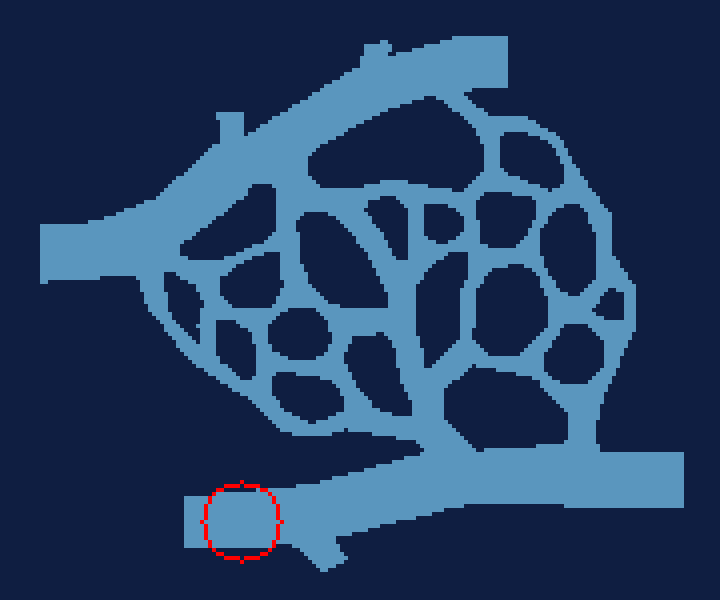
\includegraphics[clip, width=3.5cm]{figures/evaluation/procedure/capillary_upscaled.png}} & Capillary & $(180 \times 150)$ & $7169 \ (\approx 26.55\%)$ & 91.22 & 149 \\
            &&&&&\\[-1em]
            \hline
            &&&&&\\[-1em]
            \parbox[c]{3.5cm}{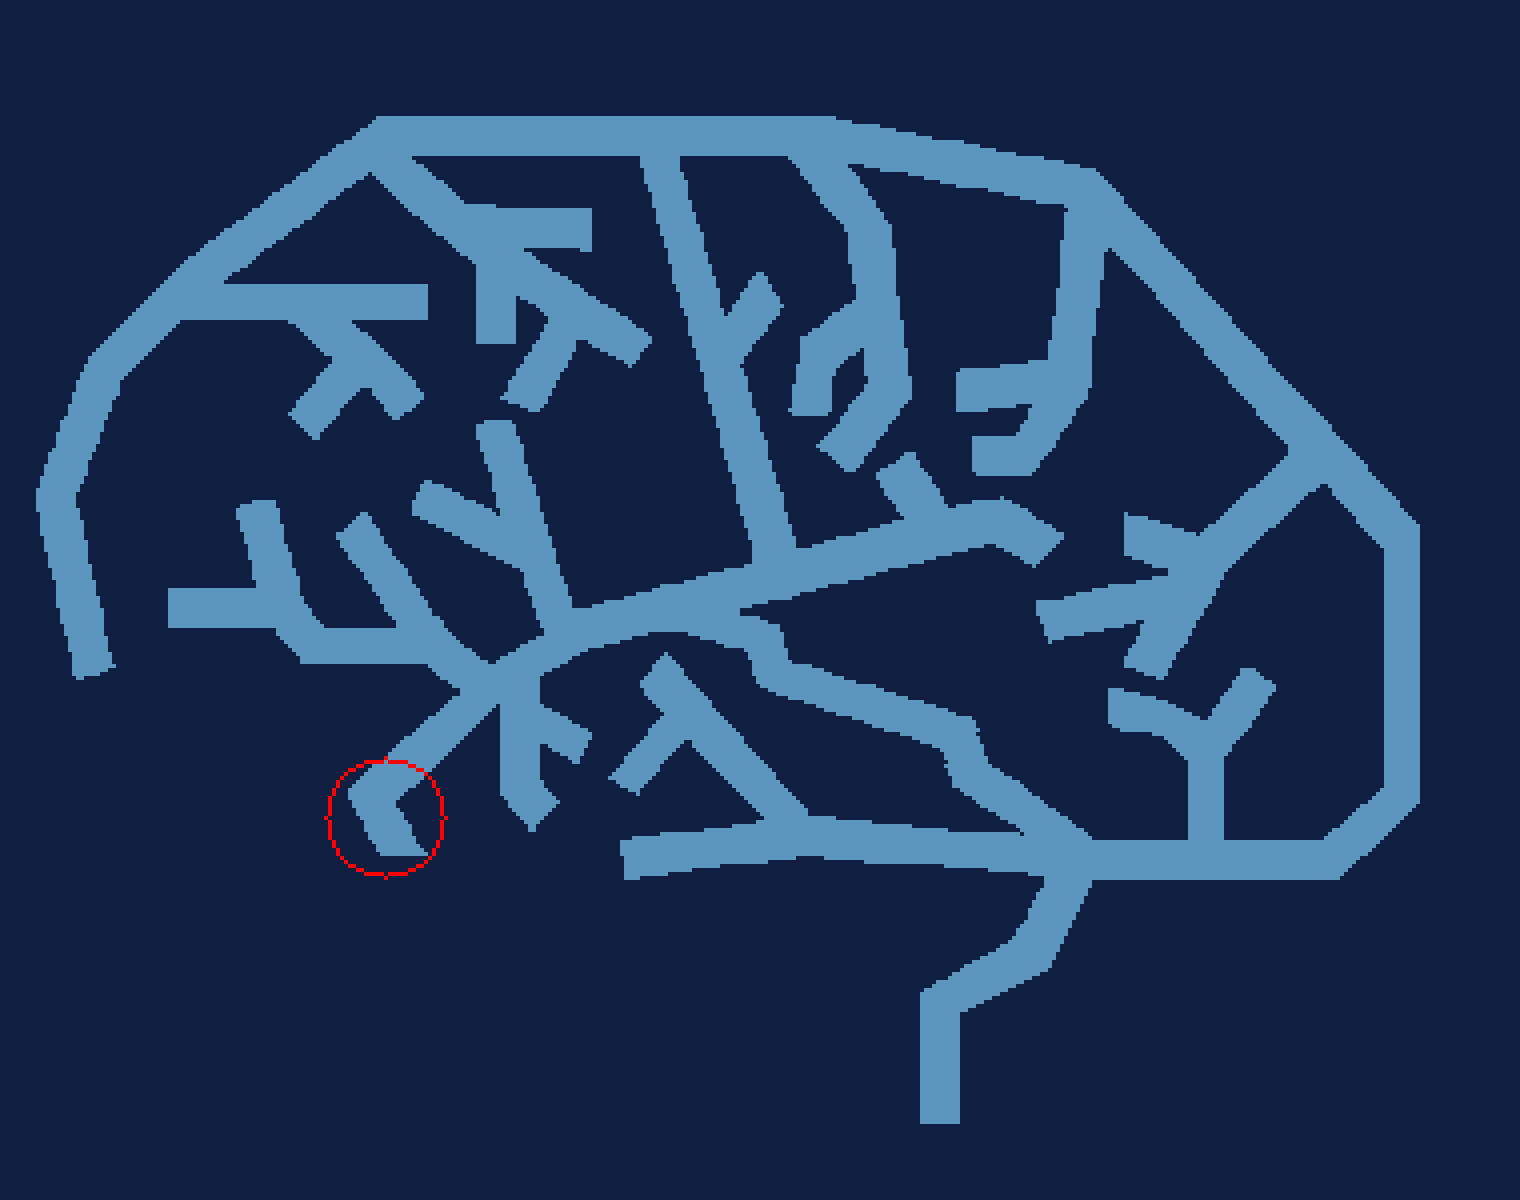
\includegraphics[clip, width=3.5cm]{figures/evaluation/procedure/brain_upscaled.png}} & Brain & $(380 \times 300)$ & $22593 \ (\approx 19.82\%)$ & 221.19 & 400 \\
            &&&&&\\[-1em]
            \hline
            &&&&&\\[-1em]
            \parbox[c]{3.5cm}{
\includegraphics[clip, width=3.5cm]{figures/evaluation/procedure/vessel_upscaled.png}} & Vessel & $(130 \times 80)$ & $4949 \ (\approx 47.59\%)$ & 77.47 & 136 \\[1cm]
            \hline
        \end{tabular}
    \end{center}
    \caption[Test Instances]{A list of our default test instances. Light blue pixels denote non-blocked pixels. The goal position is marked with a red circle. \textit{Dimension} describes the absolute size of the instance, while \textit{size} denotes the actual non-blocked area. We also included values for the average $d_{avg}$ and maximum $d_{max}$ distance between any point and the goal position.} \label{tab:TestInstances}
\end{table}

If not stated otherwise, we used 256 randomly generated particles for each episode during training. Instances are capped at a maximum of 2000 steps per episode independent of the use of dynamic episode length.

\section{Reward Generation} \label{sec:EvalReward}
We begin our experiments by analyzing which reward works best to guide particles to the goal position. Since the reward is crucial for the performance of RL algorithms, it is important to decide which reward works best to gain faster and better results in later experiments. Since we are dealing with a huge number of possible combinations in our reward system, we decide to use an iterative approach, where we first test many combinations on the easy Corridor instance and then only evaluate the promising combinations on the Vessel instance. We finally select the three best performing combinations from the Vessel instance and test them on the Brain instance. Since observation normalization can have a huge impact on training performance and directly influences reward generation in the case of intrinsic reward, we also decided to add observation normalization in the form of $x \mapsto CLIP((x - \mu)/\sigma, [-10, 10])$ into this experiment.

\paragraph{Corridor Results.}
Table TODO lists the tested reward combinations 


% \begin{table}
%     \begin{center}
%         \begin{tabular}{|c|c|c|c|c|c|n{3}{2}|n{3}{2}|}
%             \hline
%             \multicolumn{6}{|c|}{Reward Component} & \multicolumn{2}{c|}{Episode Length} \\
%             \hline
%             TP & DEL & Curiosity & Gathering & Rew Norm & Obs Norm & \multicolumn{1}{|c|}{Best} & \multicolumn{1}{c|}{Average} \\
%             \hline
%             \hline
%             x & & & & & & 135 & \\
%             x & & & & x & & \boldmath 83.78 & \\
%             & & & & & & & \\
%             & & & & & & & \\
%             & & & & & & & \\

%             \hline
%         \end{tabular}
%     \end{center}
% \end{table}

\begin{table}
    \begin{center}
        \begin{tabular}{|c|c|c|c|c|c|L|L|}
            \hline
            \multicolumn{6}{|c|}{Reward Component} & \multicolumn{2}{c|}{Episode Length} \\
            \hline
            Obs Norm & Rew Norm & TP & DEL & Curiosity & Gathering & \multicolumn{1}{|c|}{Best} & \multicolumn{1}{c|}{Average} \\
            \hline
            \hline
            & & x & & & & 135.00 & \\
            & & x & & x & & \multicolumn{1}{B{.}{.}{2, 2}|}{83.78} & \\
            & & & & & & & \\
            & & & & & & & \\
            & & & & & & & \\

            \hline
        \end{tabular}
    \end{center}
\end{table}



\section{Observations} \label{sec:EvalObs}
Observations
\section{RL Algorithms} \label{sec:EvalRLAlgorithms}
RL Algorithms
\section{Hyperparameters} \label{sec:EvalParameters}
Hyperparameters
\section{Extended Environment Models} \label{sec:EvalExtendedModels}
Extended Environment Models
\subsection{Dealing with Error} \label{sec:EvalError}
Dealing with Error
\subsection{Physical Particles} \label{sec:EvalPhysical}
Physical Particles
\section{Randomized Instances} \label{sec:EvalRandomness}
Randomized Instances
\subsection{Random Goal Positions} \label{sec:EvalRandomGoals}
Random Goal Positions
\subsection{Random Mazes} \label{sec:EvalRandomMaze}
Random Mazes
\section{Comparison to Algorithmic Approaches} \label{sec:EvalAlgorithms}
Comparison to Algorithmic Approaches